\documentclass[aspectratio=169]{beamer}



\mode<presentation>
{
\setbeamercolor{section in head/foot}{use=structure,bg=structure.fg!25!bg}

\useinnertheme{rounded}
\setbeamertemplate{frametitle}[default][center]
\setbeamertemplate{footline}[frame number]
\setbeamertemplate{itemize items}[circle]

\setbeamercolor{block title}{use=structure,fg=structure.fg,bg=structure.fg!8!bg}
\setbeamercolor{block title alerted}{use=alerted text,fg=alerted text.fg,bg=alerted text.fg!10!bg}
\setbeamercolor{block title example}{use=example text,fg=example text.fg,bg=example text.fg!05!bg}

\setbeamercolor{block body}{parent=normal text,use=block title,bg=structure.fg!8!bg}
\setbeamercolor{block body alerted}{parent=normal text,use=block title alerted,bg=block title alerted.bg!20!bg}
\setbeamercolor{block body example}{parent=normal text,use=block title example,bg=example text.fg!05!bg}

%change beamer button color
\setbeamercolor{button}{bg=white,fg=green}
\usefonttheme{professionalfonts}

%table of contents
\setbeamertemplate{section in toc}{\hspace{1.2em}{\color{blue}{$\bullet$}}~\inserttocsection\par}
}

%%%%change proof block color
\addtobeamertemplate{proof begin}{%
    \setbeamercolor{block title}{fg=orange!60!white,bg=orange!10!white}%
    \setbeamercolor{block body}{fg=black, bg=orange!10!white}%
}{}

\addtobeamertemplate{qed symbol}{%
    \color{orange!60!white}%
}

% All the usepackage will come here. No usepackage later.
\usepackage{amsfonts}
\usepackage{amsmath}
\usepackage{amssymb}
\usepackage{graphicx}
\usepackage{color}
\usepackage[mathcal]{euscript}
\usepackage{tikz}
\usepackage{pgfplots}
\pgfplotsset{compat=1.17} 
\usepackage{mathtools}
\let\algorithm\relax
\let\endalgorithm\relax
\usepackage[linesnumbered,ruled,vlined]{algorithm2e}
\newcommand\mycommfont[1]{\footnotesize\ttfamily\textcolor{gray}{#1}}
\SetCommentSty{mycommfont}
\let\oldnl\nl% Store \nl in \oldnl
\newcommand{\nonl}{\renewcommand{\nl}{\let\nl\oldnl}}% To remove line number for one line
\usepackage{braket}%%for defining set
\usepackage{subcaption}%for subtables
\usepackage{multirow}%for multirows
\usepackage{adjustbox}
\usepackage{slashbox}%%for backslash in tables
\usepackage{xspace}%for space after macro
\usepackage{soul} % for crossing out text

%%url line break
\makeatletter
\g@addto@macro{\UrlBreaks}{\UrlOrds}
\makeatother

%------reset footnote number for each slide
\AtBeginEnvironment{frame}{\setcounter{footnote}{0}}

%%for long division---
\usepackage{longdivision}
\usepackage{scalerel}
\setcounter{MaxMatrixCols}{20}
\newcommand{\longdiv}{\smash{\mkern-0.43mu\vstretch{1.31}{\hstretch{.7}{)}}\mkern-5.2mu\vstretch{1.31}{\hstretch{.7}{)}}}}
%%----

%--------------------New functions---------

\def \NN {{\mathbb N}}
\def \CC {{\mathbb C}}
\def \RR {{\mathbb R}}
\def \QQ {{\mathbb Q}}
\def \H {{\mathbb H}}
\def \FF {{\mathbb F}}
\def \ZZ {{\mathbb Z}}
\def \a {{\mathfrak a}}
\def \b {{\mathfrak b}}
\def \p {{\mathfrak p}}
\def \Pf {{\mathfrak P}}

\def \tta {{\texttt A}}
\def \ttb {{\texttt B}}
\def \ttc {{\texttt C}}
\def \ttd {{\texttt D}}
\def \ttf {{\texttt F}}
\def \m {{\mathfrak m}}

\DeclareMathOperator*{\argmax}{arg\,max}%%define argmax
\DeclareMathOperator*{\argmin}{arg\,min}%%define argmin

\newcommand{\mo}{\textrm{~mod~}}
\newcommand{\ord}[1]{\textrm{ord}(#1)}
\newcommand{\node}[2]{``\texttt{#1} \ (#2)\textnormal{''}}
\newcommand{\picsrc}[1]{\text{{\tiny src: \url{#1}}}}
\newcommand{\cov}[1]{\textrm{Cov}{\left(#1\right)}}
\newcommand{\var}[1]{\textrm{Var}{\left(#1\right)}}
\newcommand{\ex}[1]{\textrm{E}\left[#1\right]}
\newcommand{\wt}[1]{\textrm{wt}\left(#1\right)}
\newcommand{\dis}[1]{\textrm{dis}\left(#1\right)}

%-----------------Datasets--------------
\newcommand{\datafixone}{\textit{Fixed dataset A}\xspace}
\newcommand{\datafixtwo}{\textit{Fixed dataset B}\xspace}
\newcommand{\dataranone}{\textit{Random plaintext dataset}\xspace}
\newcommand{\datarantwo}{\textit{Random dataset}\xspace}

%--------------------End of New Functions----

\setbeamertemplate{footline}[frame number]

%change beamer button color
\setbeamercolor{button}{bg=white,fg=green}

% ----------------------------------------------

\title{{\Huge \SectionName} \texorpdfstring{\\ \vspace{1cm} {\normalsize SECTION \SectionNumber}}{}}

% \author{Jakub Breier\texorpdfstring{\\TTControl \vspace{1cm}\\}{}Xiaolu Hou\texorpdfstring{\\ Slovak University of Technology}{}}
\date{}

\AtBeginSubsection[] {
  \begin{frame}<beamer>
    \frametitle{Outline}
    \tableofcontents[currentsection,currentsubsection]
  \end{frame}
}




\def \SectionName {{Course Conclusion}}
\def \SectionNumber {{6}}
\def \VideoName {{Thank You and Contact Information}}
\def \VideoNumber {{6.3}}


\begin{document}
\maketitle

\begin{frame}{}
\LARGE{
\begin{center}
     \usebeamercolor[fg]{frametitle}{\VideoName}
\end{center}}
\vspace{1cm}
\normalsize{
\begin{center}
     \usebeamercolor[fg]{frametitle}{Video Number \VideoNumber}
\end{center}}
\end{frame}

\begin{frame}{Textbook and dataset}
    \begin{columns}[T] % align columns
\begin{column}{.6\textwidth}
        \begin{itemize}
        \item Textbook: Cryptography and Embedded Systems Security, 2024
        \begin{center}
        \url{https://link.springer.com/book/9783031622045}
        \end{center}
        \item Free version
        \begin{center}
        \url{https://jbreier.com/assets/pdf/Cryptography_and_Embedded_Systems_Security.pdf}
        \end{center}
        \item Dataset, script and experimental results
        \begin{center}
            \url{https://github.com/XIAOLUHOU/SCA-measurements-and-analysis----Experimental-results-for-textbook}
        \end{center}
    \end{itemize}
\end{column}%
\hfill%
\begin{column}{.5\textwidth}
\begin{figure}
    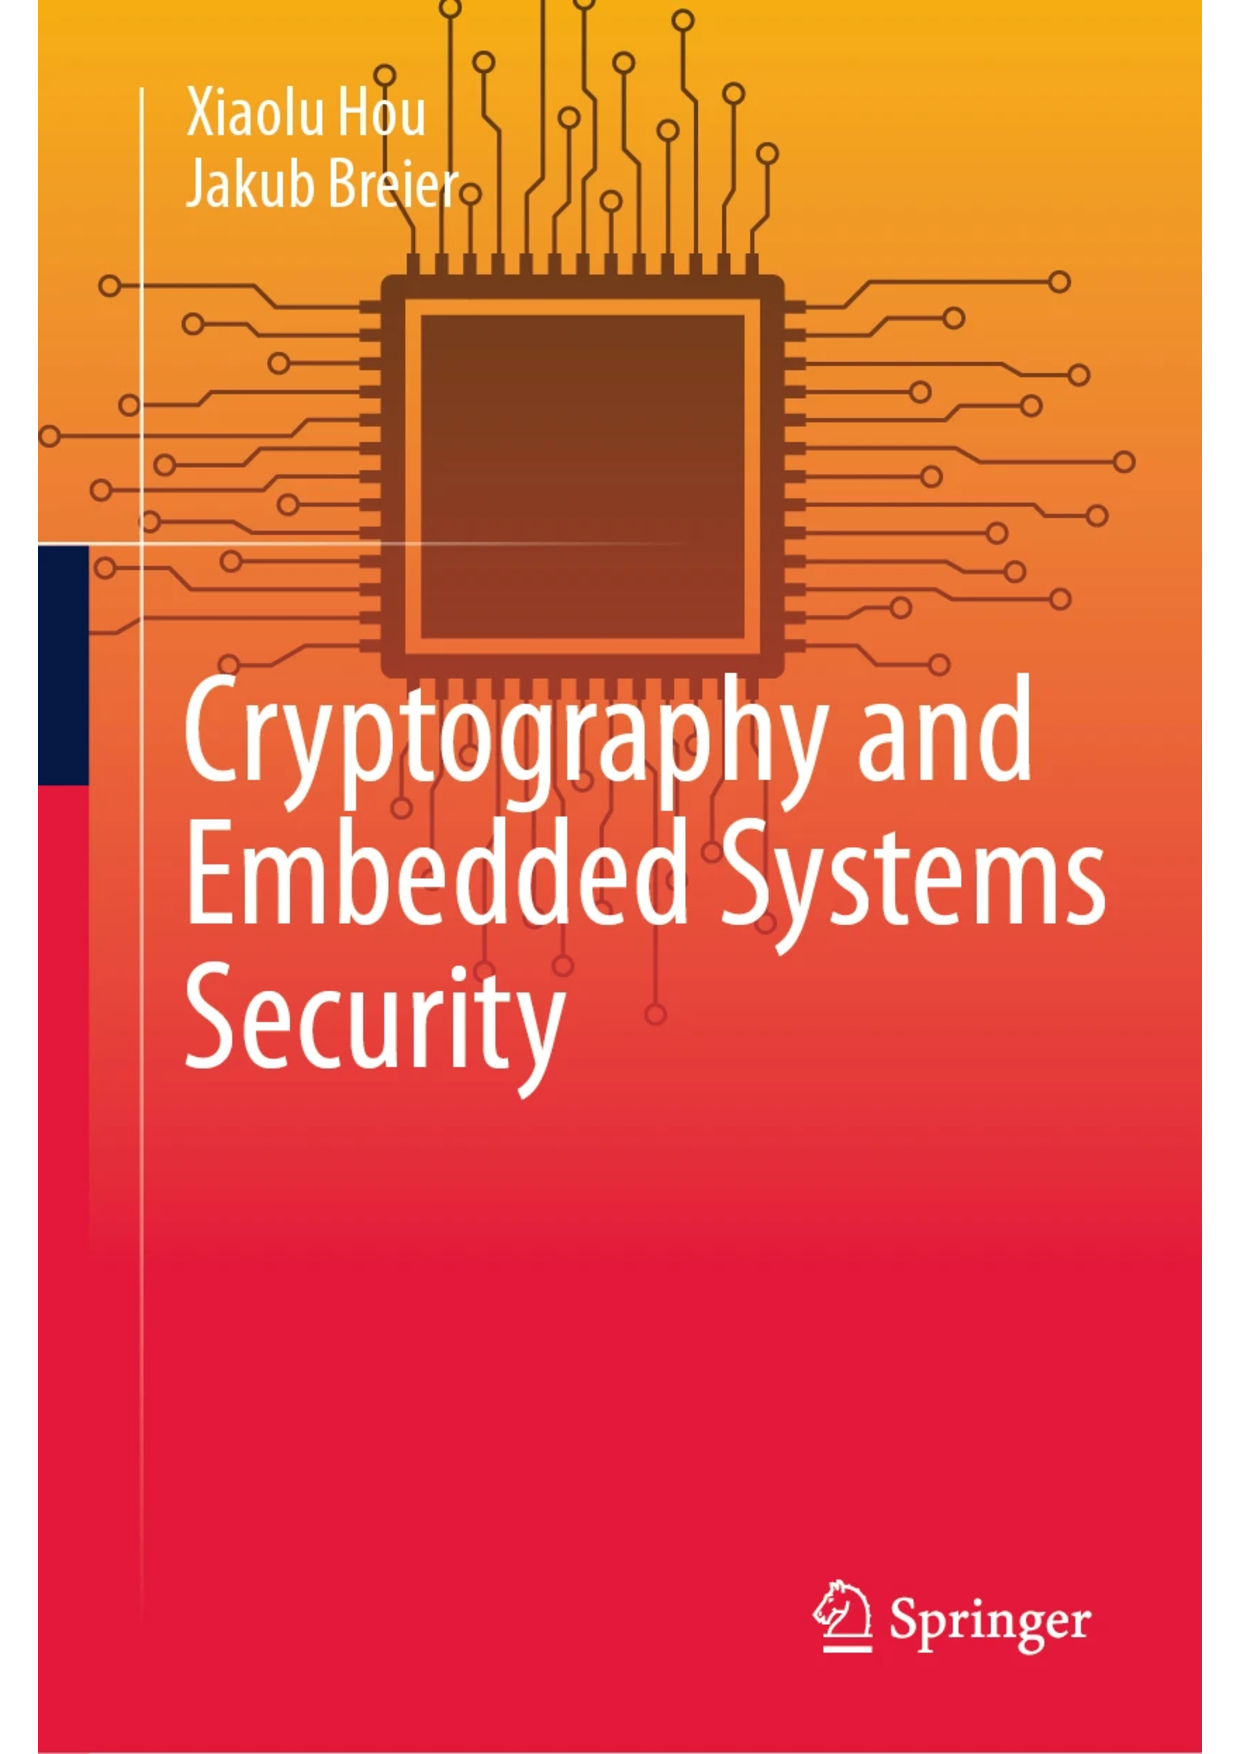
\includegraphics[width=0.7\textwidth]{fig/Textbook.pdf}
\end{figure}
\end{column}%
\end{columns}
\end{frame}

\begin{frame}{About Dr. Hou}
\begin{columns}[T] % align columns
\begin{column}{.7\textwidth}
\begin{itemize}
        \item Assistant professor at Faculty of Informatics and Information Technologies, Slovak University of Technology
        \item Research interest: hardware attacks and countermeasures on cryptographic implementations and neural networks
        \item Google Scholar: \url{https://scholar.google.com.sg/citations?user=-u5TP78AAAAJ&hl=en&oi=ao}
        \item Webpage: \url{https://xiaoluhou.github.io/}
        \item Contact info: houxiaolu.email@gmail.com
    \end{itemize}

\includegraphics[width=3cm]{fig/EU-flag-and-Marie-Curie-Logo.jpg} \hspace*{0.75cm}~%

\includegraphics[width=1.5cm]{fig/SAS_logo.png}\hspace*{0.75cm}~%

\includegraphics[width=3cm]{fig/saspro2_logo.png}
\end{column}%
\hfill%
\begin{column}{.5\textwidth}
\begin{figure}
    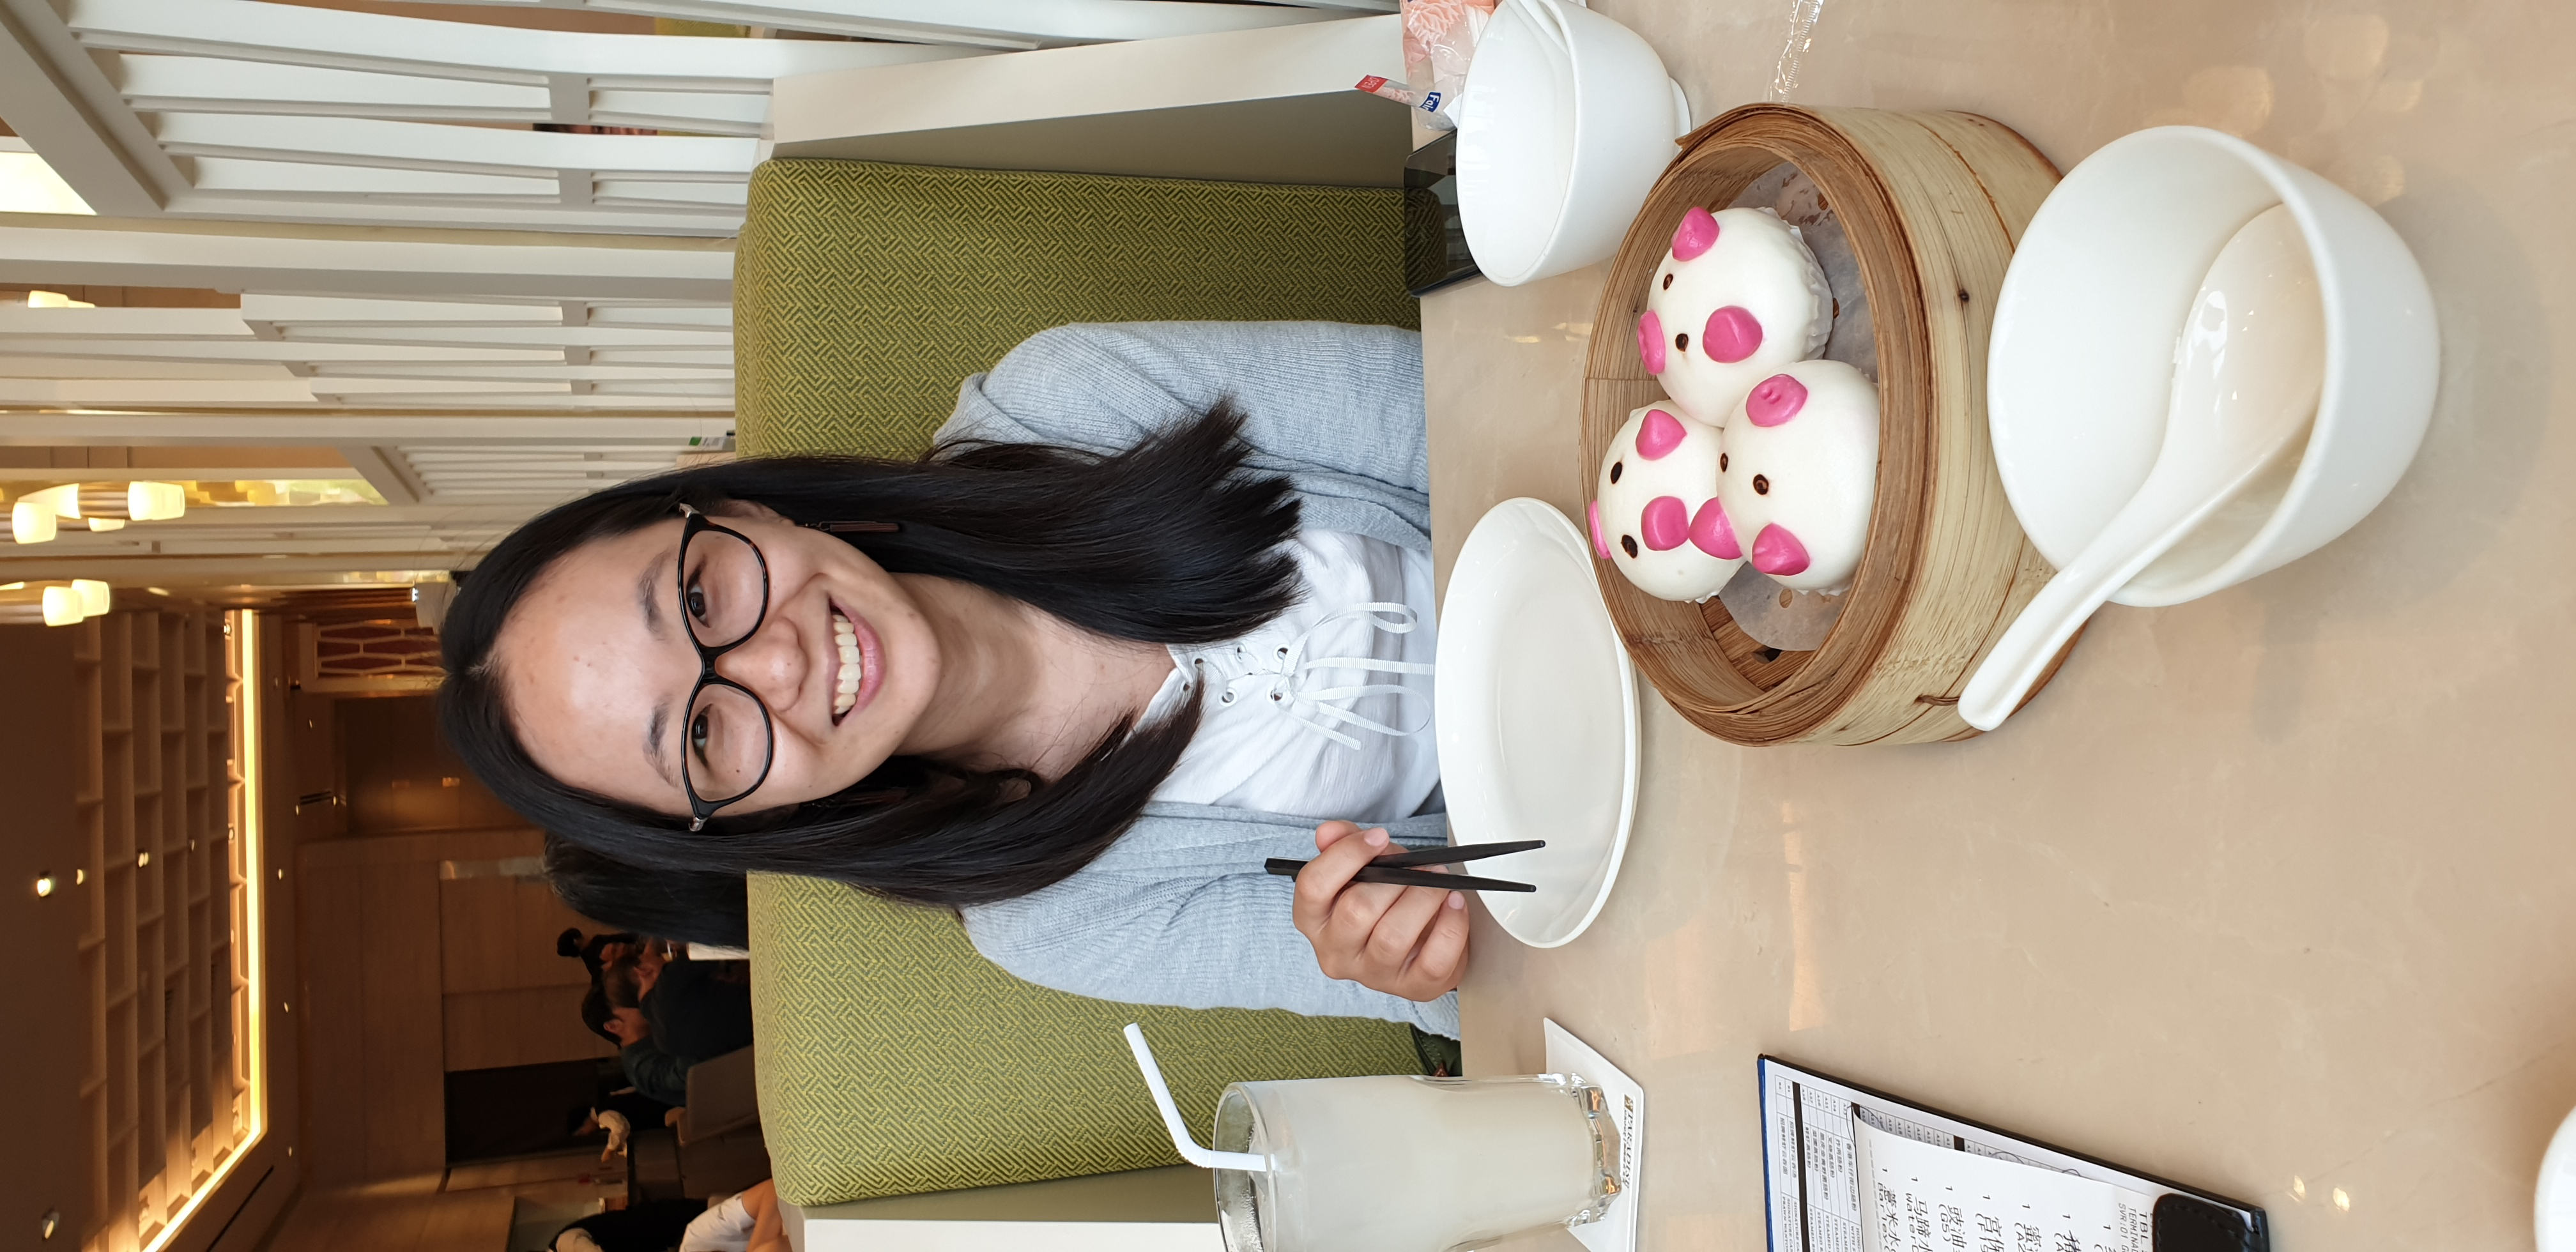
\includegraphics[width=0.9\textwidth, angle=-90]{fig/Xiaolu.jpg}
\end{figure}
\end{column}%
\end{columns}
\end{frame}

\begin{frame}{About Dr. Breier}
\begin{columns}[T] 
\begin{column}{.7\textwidth}
    \begin{itemize}
        \item Senior Cyber Security Manager at TTControl GmbH, Vienna, Austria
        \item Researching, evaluating, and implementing hardware security, automotive security, and cryptography
        \item Google Scholar: \url{https://scholar.google.com/citations?user=LOENK6IAAAAJ&hl=en}
        \item Webpage: \url{https://jbreier.com}
        \item Contact info: jakub.breier@gmail.com
    \end{itemize}
\end{column}
\begin{column}{.3\textwidth}
\begin{figure}
    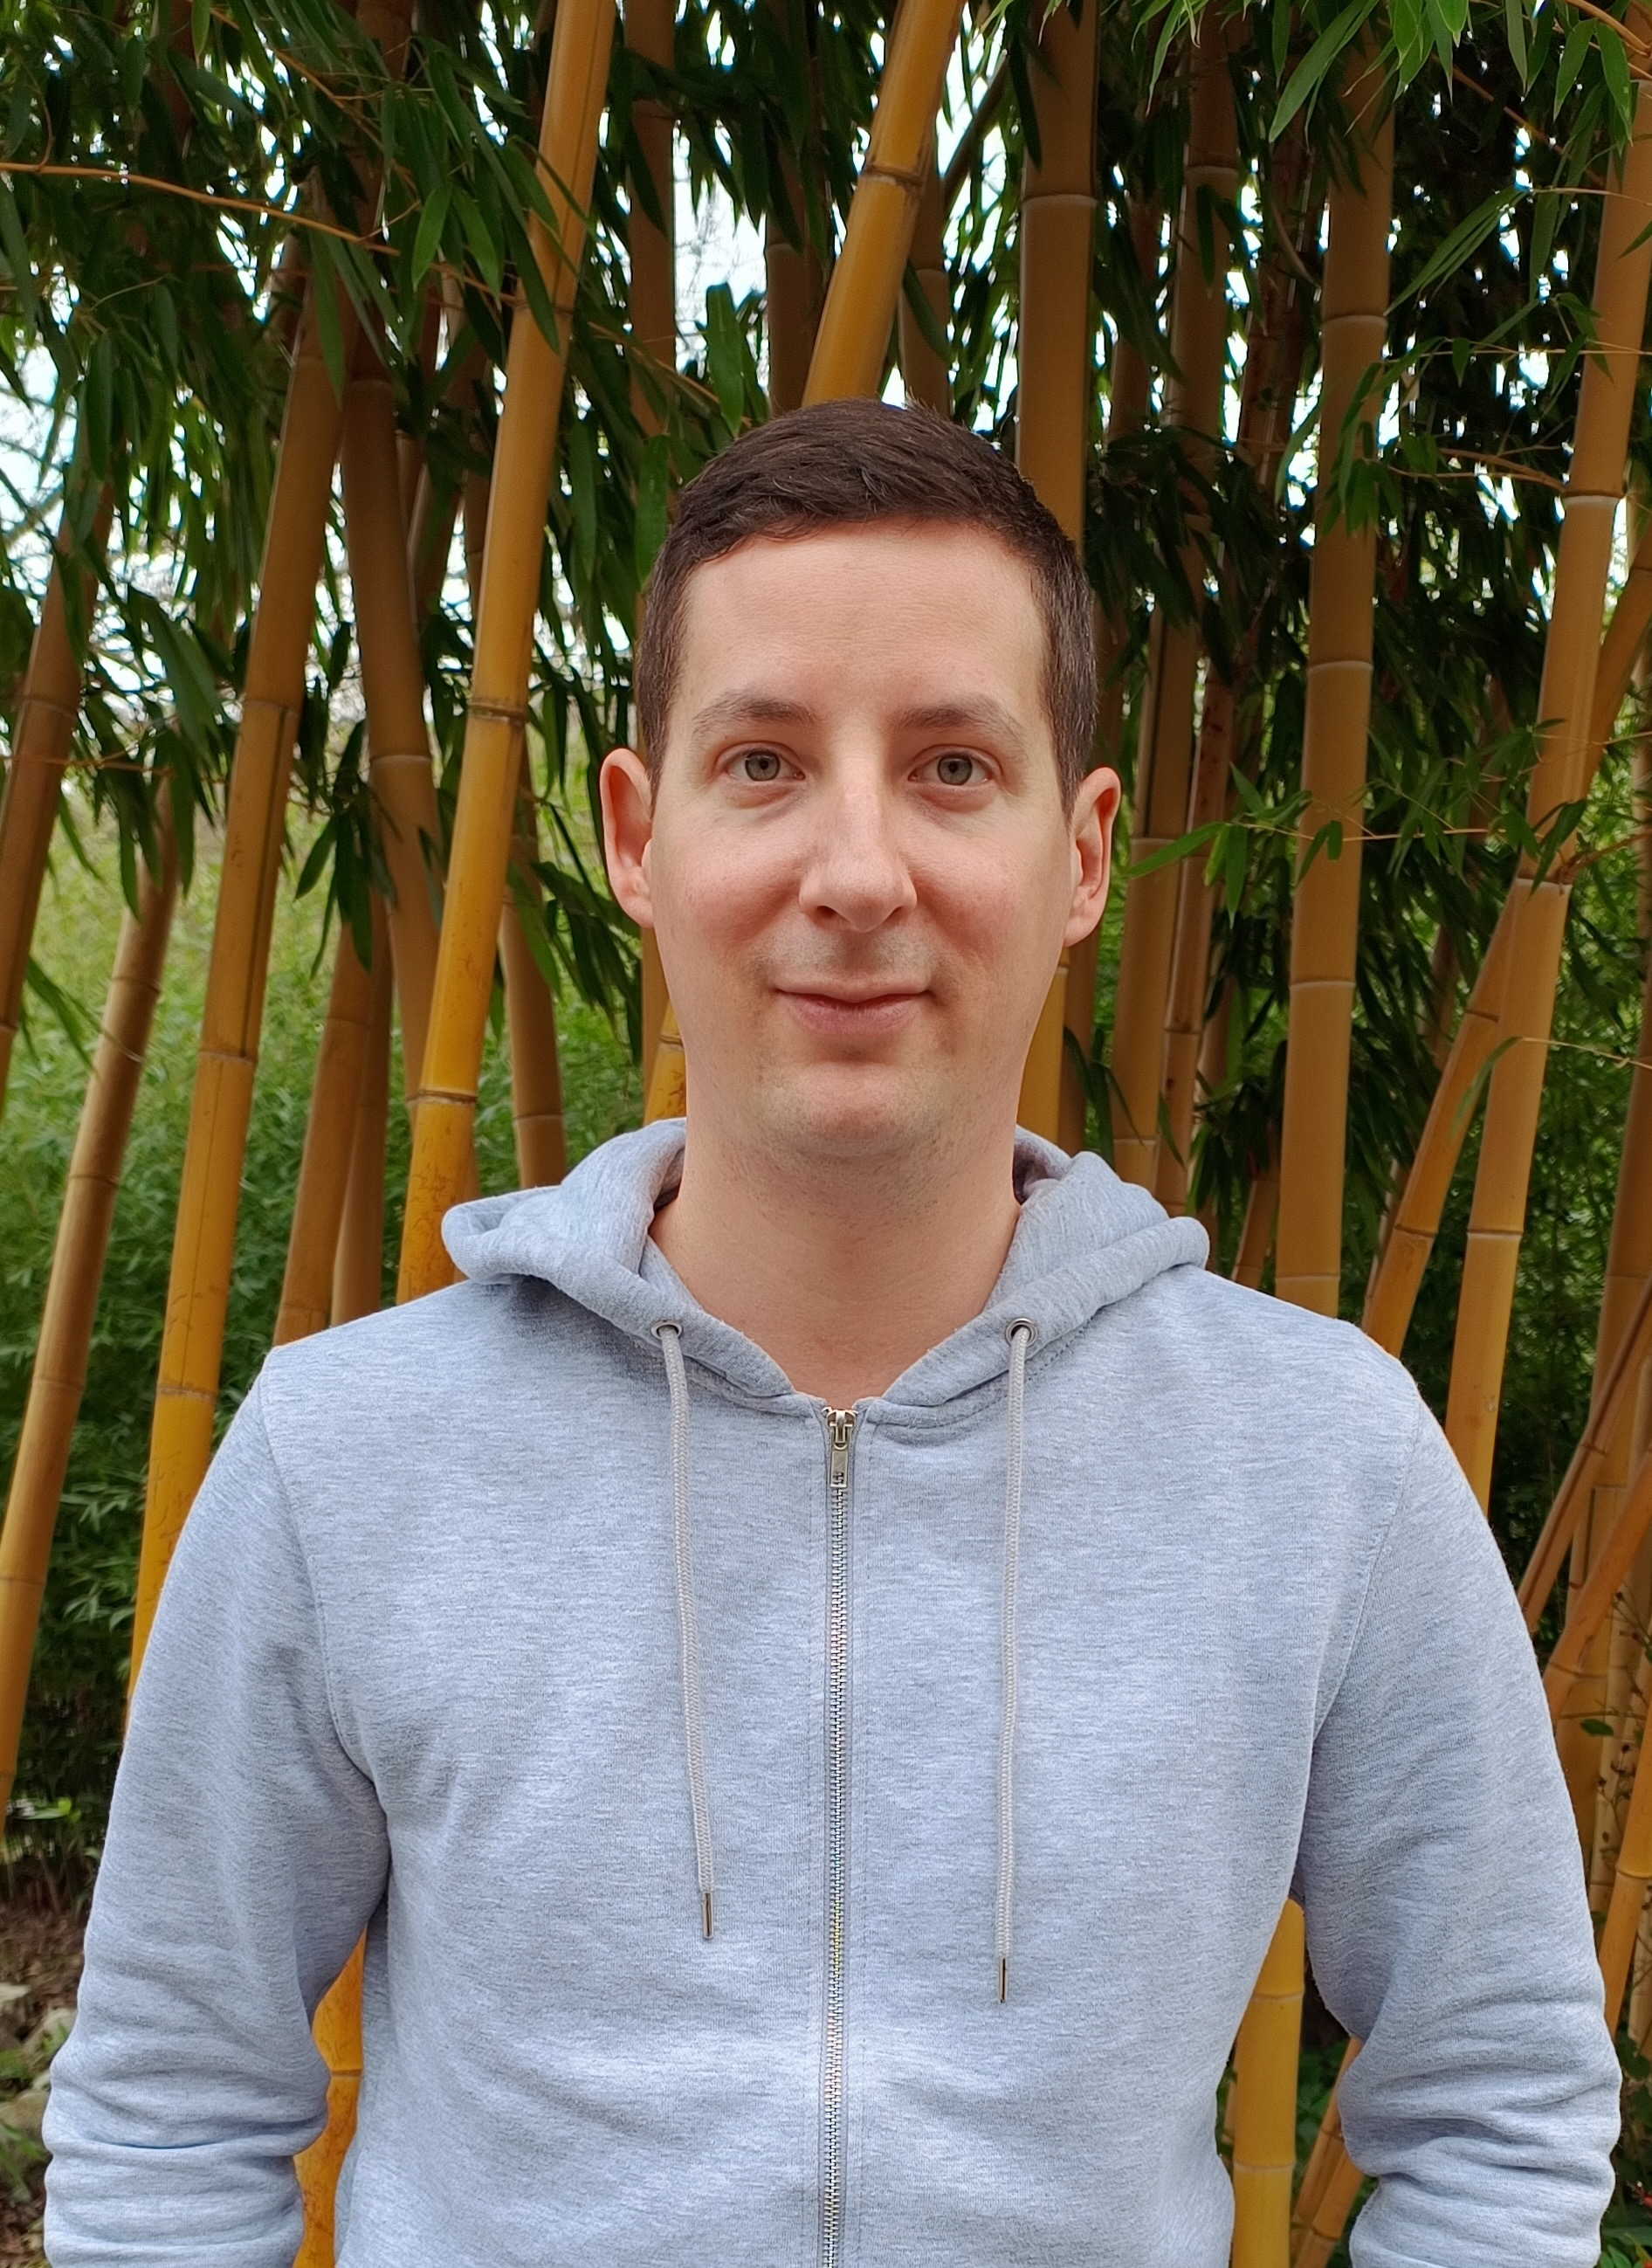
\includegraphics[width=0.9\textwidth]{fig/jakub.jpeg}
\end{figure}
\end{column}
\end{columns}
\end{frame}



\begin{frame}{PhD and Master thesis topics}
\begin{itemize}
    \item We are both looking for motivated PhD and master's students
    \item Having completed the course, you now possess a solid foundation to embark on your research.
\end{itemize}
Topics:
    \begin{itemize}
        \item Fault attacks and countermeasures
        \begin{itemize}
            \item Cryptographic implementations
            \item Neural networks
        \end{itemize}
        \item Side-channel attacks and countermeasures
        \begin{itemize}
            \item Cryptographic implementations
            \item Neural networks
            \item AI for side-channel attacks
        \end{itemize}
    \end{itemize}
\vfill

Contact info: houxiaolu.email@gmail.com, jakub.breier@gmail.com
\end{frame}

\end{document}